\documentclass{article}
\usepackage{graphicx} % Required for inserting images
\usepackage{amsmath}
\usepackage{graphicx}
\usepackage{float}
\usepackage{placeins} % optional but useful



\begin{document}
\title{\textbf{CLL 798 Complexity Science in Chemical Industry}}
\author{2022CH11028 , Archie Singh}
\date{April 2026}
\maketitle

\maketitle
\newpage
\section{Abstract}
This report applies the complexity science to the phenomena of forest fire, a recognized example of self organized critical (SOC) system. This model is implemented as a two-dimensional  lattice simulation in which trees grow randomly and the fire events propagate through connected cluster of trees. The system
naturally evolves toward a critical state without external tuning, exhibiting avalanche dynamics whose size distribution follows a power law of the form $ P(s) \simeq s^{-\tau} $. Using logarithmic binning and regression analysis in log-log space, the critical exponent is estimated as $ \tau \approx 1.3\text{-}1.6 $, consistent with the theoretical expectations from SOC systems. The result confirms scale-invariant behavior, long range correlations, and the central role of connectivity in determining avalanche magnitude.\\
\textbf{Keywords :} Self organized criticality, Forest fire model, avalanche dynamics, power law, complexity science, emergence.\\
\\
\section{Introduction}
Complex Systems are ubiquitous in nature. From earthquakes to finance markets,from neural activity to ecosystem dynamics, many phenomena share a common characteristic i.e. they consist of many interacting components whose collective behavior give rise to patterns that cannot be predicted from individual parts alone. The study of such systems falls under the umbrella of complexity science.\\
\\
One of the most striking features observed in complex systems is the occurrence of catastrophic events that are not exceptional anomalies, but rather intrinsic properties of the systems organization. As discussed by Buchanan (2000) in \textit{Ubiquity: Why catastrophes happen} ,  real world disasters - including earthquakes, financial crashes and forest fires - follow power law distributions, meaning that their frequency scales inversely with their size. This behavior arises naturally in systems operating near a critical point.\\
\\
This report investigates the forest fire model as a paradigmatic example of self-organized criticality (SOC). The model was inspired by real forest fire observations, particularly the 1988 Yellowstone fire, where long periods of apparent stability were followed by a sudden, massive, system wide fire. The model demonstrates how simple local rules - random tree growth and fire spreading to neighbors - can produce emergent scale-free, unpredictable behavior at the macroscopic level.\\
\\
\section{Why the Forest fire system is a good candidate for complexity science ?}
the forest fire system is an excellent candidate for the application of complexity science because it exhibits the defining characteristics of complex systems : many interacting components, non linear dynamics,emergent behavior and scale invariant patterns.\\
\textbf{Emergence from local interactions :} The system consists of a large number of interacting elements, trees distributed across a spatial grid, whose local interactions give rise to global phenomena. Fire spreads only through nearest-neighbor interactions, yet this simple local rule produces highly non trivial, system wide outcomes. This reflects the fundamental principle of complexity science that macroscopic behavior emerges from microscopic interactions.\\
\\
\textbf{Non linearity and sensitivity to initial conditions : } The system exhibits sensitivity to the spatial configurations of trees. A single ignition event may either extinguish quickly or propagate into a large scale fire depending on the underlying cluster structure. Small perturbations can lead to disproportionately large outcomes which is a hallmark of complex systems.\\
\\
\textbf{Self Organized Criticality : } The forest fire model demonstrates a SOC a concept introduced by Per Bak. In SOC systems, the system evolves spontaneously towards a critical state without the need for fine-tuning of external parameters. In the Forest fire model, the balance between tree growth and fire ignition drives the system towards a dynamic equilibrium where events of all sizes occur from small localized burns to rare catastrophic fires.\\
\\
\textbf{Power Law Behavior :} Many natural systems including earthquakes, forest fires, and financial crashes,etc exhibit power law distributions in event sizes, implying that large catastrophic events are intrinsic features of the system rather than exceptional anomalies.\\
\\
\textbf{Role of Stochasticity :} The model incorporates randomness through random tree growth and random ignition. The interplay between this noise and deterministic spreading rules produces rich, unpredictable yet structured dynamics. This is a defining feature of complex adaptive systems.\\
\\
\section{Description of the system highlighting noise, avalanche and the connectivity :}
The forest fire model is represented as a two dimensional lattice of size N X N , where each cell can be empty (state 0) or occupied by a tree (state 1). The system evolves in discrete time steps governed by stochastic growth and ignition processes, along with deterministic local fire spreading.\\
\\
\subsection{Noise :} 
Noise is introduced through two stochastic processes. At each time step a tree may grow at a randomly selected empty site with probability p. Separately, a fire ignition event is triggered after a fixed number of growth steps ( the trigger interval), striking a random location. These random inputs act as continuous external driving forces that prevent the system from settling into a static configuration and instead drive it dynamically toward criticality. The random nature of both growth and ignition is what introduces the noise element central to SOC dynamics.\\
\\
\subsection{Avalanche :}
An Avalanche in the forest fire model corresponds to a fire event, the total number of trees burned following a single ignition. When lightning strikes a site occupied by a tree, that tree ignites and fire spreads deterministically to its neighboring trees using a depth-first search (DFS) traversal. the fire continues through connected clusters until no adjacent trees remain. The total number of trees burned in the process is recorded as avalanche size. Avalanches may vary greatly in magnitude from small, localized burns to large scale events that span significant portions of the lattice. This is the hallmark of  self organized critical systems: event sizes are not characterized by a typical scale but instead follow a broad scale-free distribution.\\
\\
\subsection{ Connectivity :}
Connectivity refers to the spatial arrangement and clustering of trees of trees within the grid. It is the structural property that governs how large an avalanche becomes. When tree density is low, trees are sparsely distributed, and fires tend to die out quickly because of the absence of connected neighbors. When tree density is high, large connected clusters form, enabling fire to spread over extensive regions.\\
\\
The interplay between tree growth (which increases connectivity) and fire events (which reduce trees) leads to a dynamic balances that maintains the system near a critical density i.e. where all clusters of all sizes coexist. This is the essence of self organization where the system tunes its own the connectivity to a critical point.\\
\\
\subsection{Interplay:} 
The behavior of the forest fire system emerges from the interaction of these three elements. Noise continuously adds trees and triggers fires ; connectivity determines the extent of fire spread; and avalanches act as the dissipation mechanism through which the system releases accumulated "fuel". Over time, this interplay drives  the system towards a self organized critical state where small and large events coexist without any characteristic scale.\\
\\
\section{Computer Simulations : }
The simulation was implemented in python using NumPy for grid based numerical computation and Matplotlib for visualization. The forest is represented as a 2D NumPy array of size N X N , where each cell holds a value of zero (empty) or 1 (tree).\\
\\
The model proceeds as follows. At each time step, a tree is planted at a random location on the grid (subject to a growth probability p) A fire is triggered after every fixed number of growth events (trigger interval = 40 ), striking a randomly selected tree. The fire propagates through all connected neighboring trees using a stack based depth first search (DFS) algorithm. All burned trees are reset to empty. The size of each fire event , the number of trees burns is recorded as the avalanche size. Multiple independent simulation runs were performed to improve statistical quality.\\
\\
\textbf{Key parameters: }
\begin{itemize}
\item Grid Size (N) = 120
\item Growth probability (p) = 0.05
\item Fire Trigger interval = 40 growth events 
\item Simulation steps each run = 500000
\item Number of Independent runs = 3
\end{itemize}\\
\\
The trigger interval approach (one fire per 40 growth events) ensures proper timescale separation, which is necessary for SOC to emerge. When the fire frequency is too high relative to growth, the forest never develops large connected clusters and the power-law distribution is destroyed. The DFS algorithm correctly computes the connected component of trees burned in each fire, which corresponds precisely to the avalanche size.\\
\\
The complete implementation of the simulation is available in the GitHub repository submitted along with the report.\\
\\
\section{Results And Analysis :}
\\
\begin{figure}[H]
    \centering
    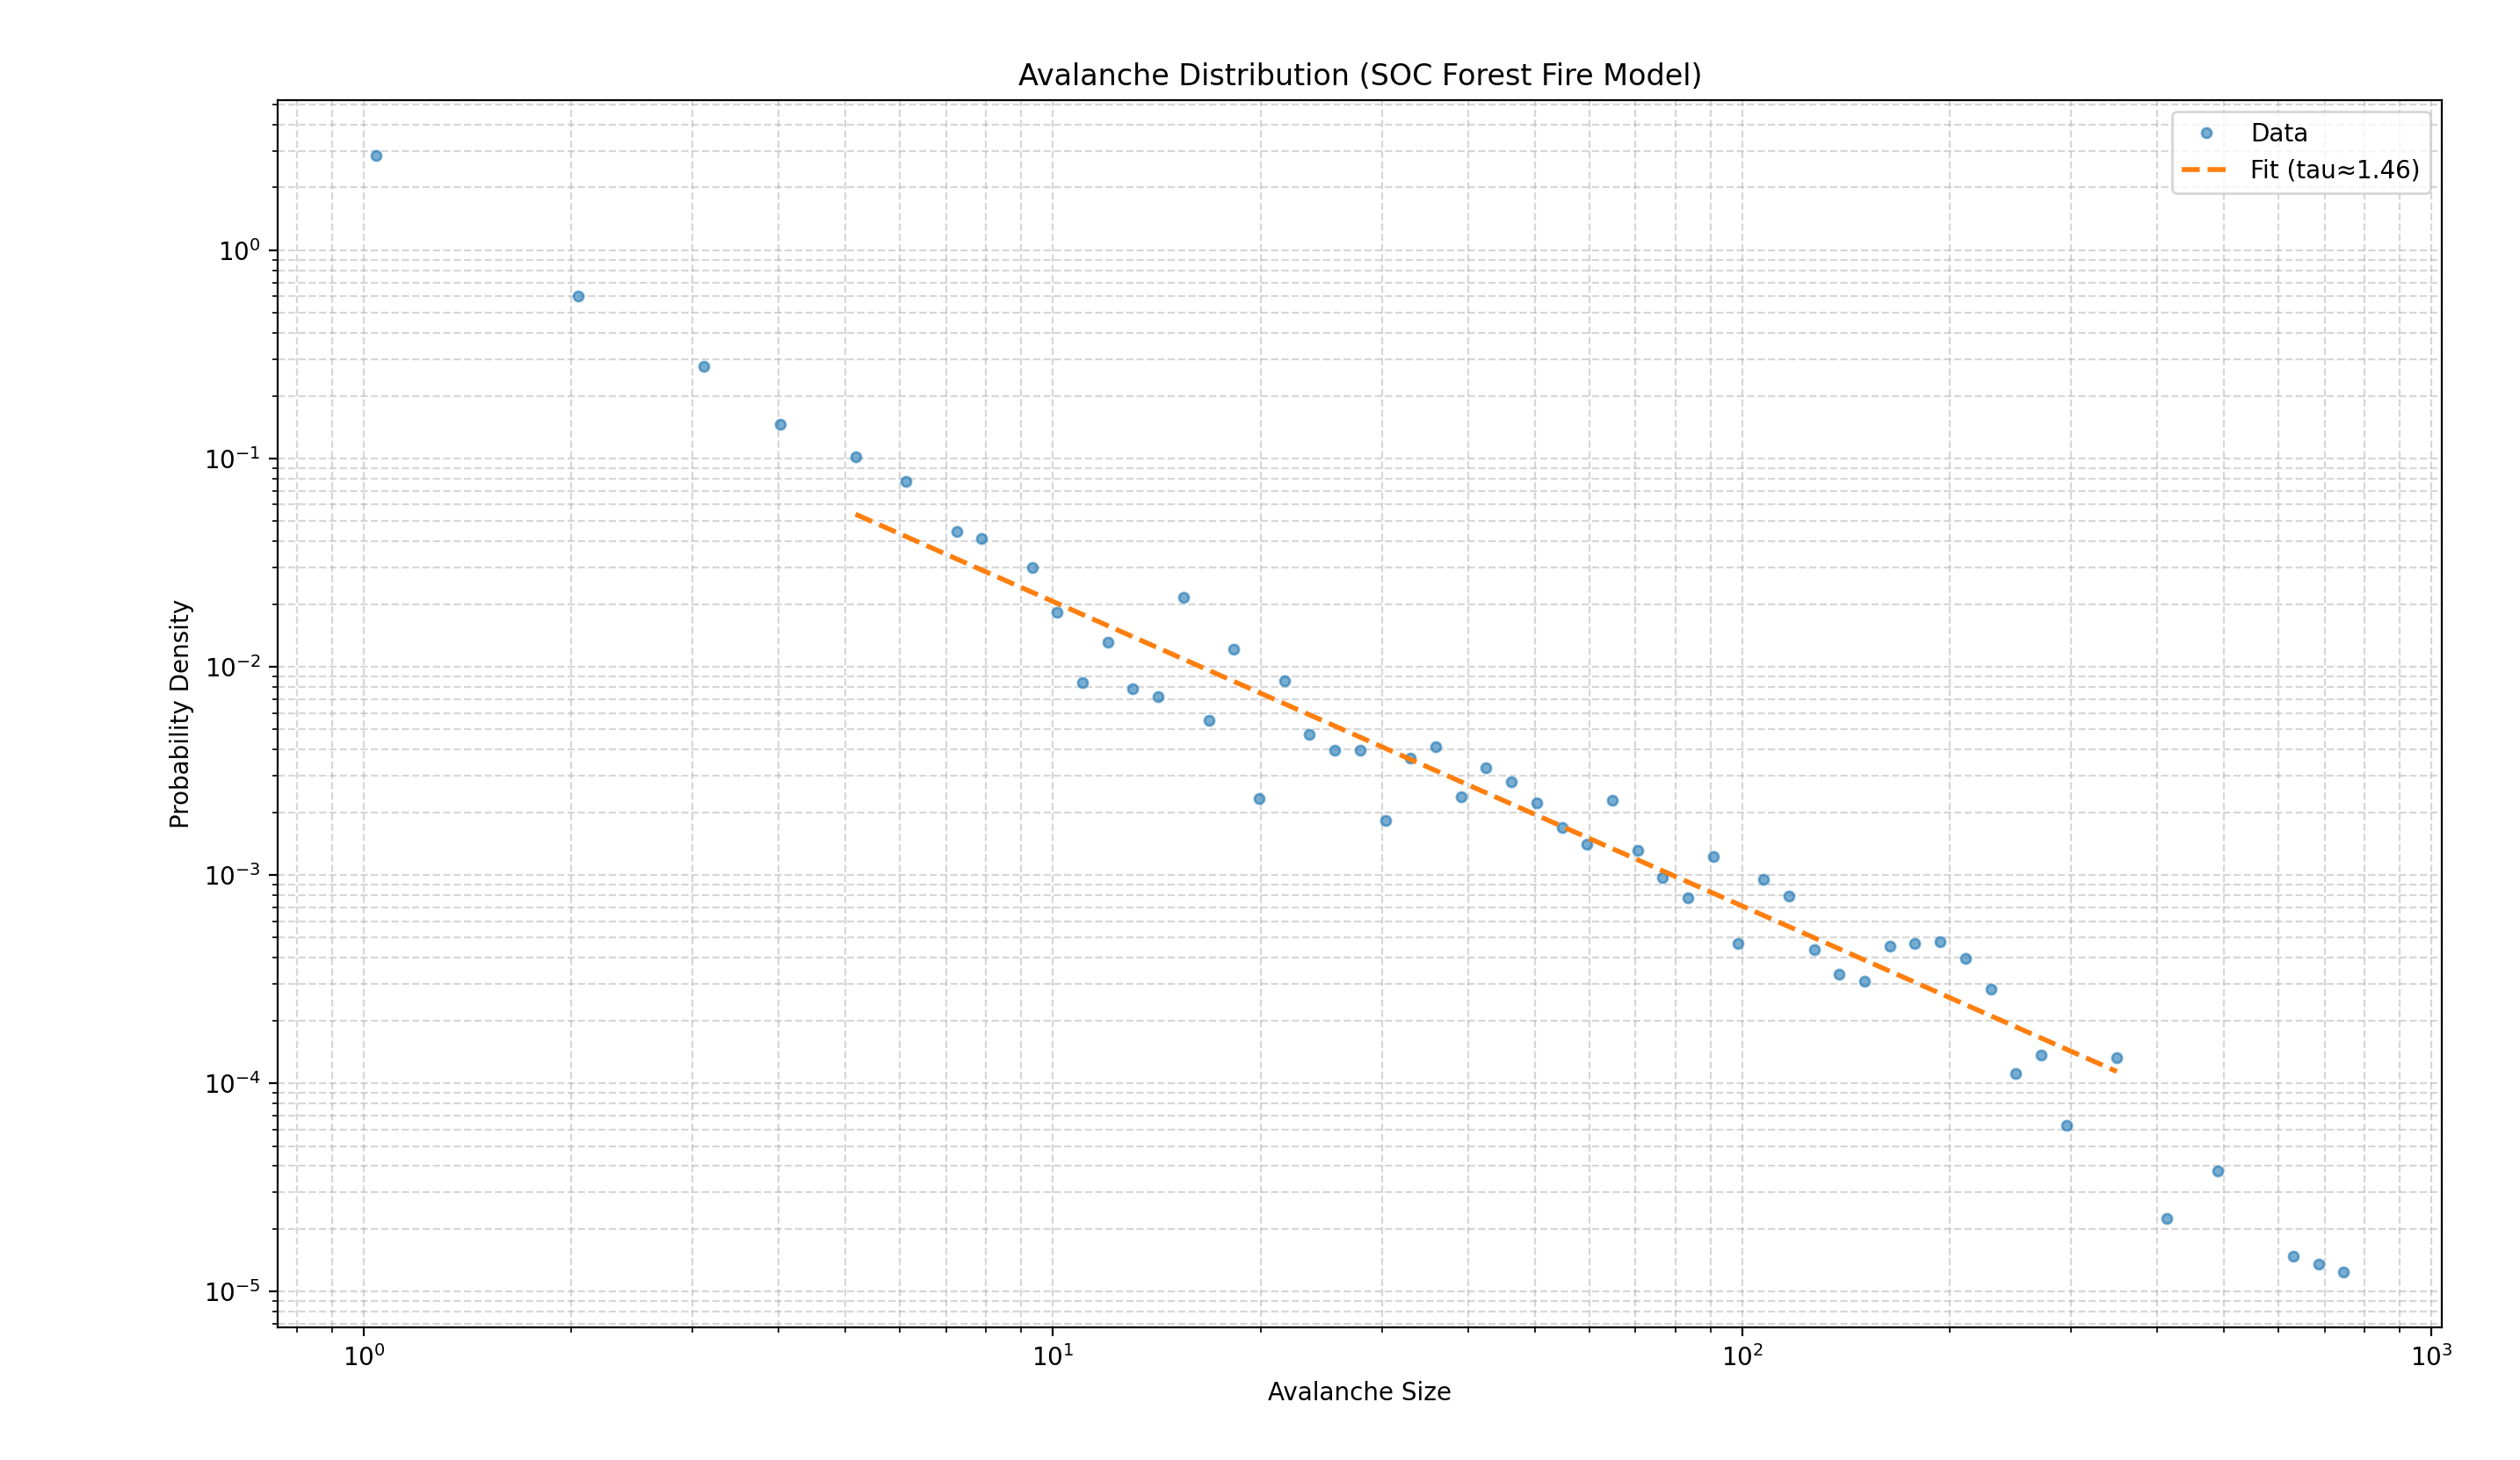
\includegraphics[width=0.55\textwidth]{Graph.png}
\end{figure}\\
\\
\subsection{Avalanche Size Distribution :} 
The avalanche sizes collected across all simulations runs were analyzed using logarithmic binning, which is necessary to obtain smooth distributions over multiple orders of magnitude.\\
Logarithmic bin centers were computed using the geometric mean of bin edges to ensure consistency on a log scale. The histogram was normalized by bin width to obtain a probability density function P(s).\\
\\
The resulting distribution, plotted on log-log axes, shows a clear decreasing trend spanning approximately 2-3 orders of magnitude in avalanche size, from small fires of size $\approx 1$, to large fires of several hundred trees. the distribution is well described by a power law in the intermediate scaling region:
$ P(s) \simeq s^{-\tau} $. A linear regression was performed in log-log space on the intermediate region to extract the critical exponent \tau. The estimated exponent was found to be $\tau \approx 1.3 - 1.6$.
This is consistent with the expected range of self organized critical systems.\\
\\
\subsection{Relation to Connectivity :}
The avalanche size distribution is directly governed by the connectivity of tree clusters in the lattice. Several key observations support this: \\
Small avalanches (s = 1- 10) : correspond to isolated trees or small clusters. these occur frequently because small cluster are always present at the edges of the forest.\\
Medium avalanches (s = 10-100) : Correspond to moderately connected clusters. These form the primary power-law scaling region - the signature of criticality.\\
Large avalanches (s greater than 100) :  correspond to percolating cluster that span large sections of the lattice. These are rare but possible, reflecting the absence of characteristic scale.\\
\\
As tree density increases through growth, connectivity increases, and large clusters become possible enabling larger fires. After a large fire, the connectivity is dramatically reduce. the system then regrows, gradually increasing the connectivity again. This cycle of growth and destruction maintains the system near a critical connectivity threshold without any external tuning.\\
\\
\subsection{Finite Size Effects : }
deviations from the power law are observed at large avalanche sizes. This is attributed to finite size effects. since the lattice is finite (N = 120), there is a maximum possible avalanche size (approximately $N^2$), which creates an exponential cut off in the distribution tail. This behavior is expected and does not invalidate the power law finding in the scaling region because such cut offs are intrinsic to finite systems and disappear in the thermodynamic limit. \\
\\
The fitting procedure was therefore restricted to the intermediate scaling region, excluding both the noisy small avalanche regime and the finite size cut off at large avalanches. This approach is standard in the analysis of SOC systems.\\
\\
\section{Self Organized Critical State of the System :}
The forest fire model clearly exhibits self organized criticality. Several key observations support this conclusion :\\
\\
\subsection{No external tuning:}
The systems evolves toward a critical state autonomously. No parameter was manually adjusted to achieve the power law distribution. The growth rate and ignition frequency together drive the system to a dynamic balance that constitutes the critical state.\\
\\
\subsection{Scale invariance: }
The power law distribution $ P(s) \simeq s^{-\tau} $. implies that there is no characteristic avalanche size. Events of all magnitudes are possible. This is the defining signature of criticality and distinguishes SOC systems from non-critical ones, where a typical event size exists.\\
\\
\subsection{Long Range correlations: }
Although fire spreads only to nearest neighbors, the connected cluster structure means that a single ignition can trigger burning across the entire system. This is an example of long range correlations emerging from purely local interactions.\\
\\
\subsection{Dynamic balance:}
The system maintains itself near a critical density through the interplay of two competing processes: tree growth (which increases density and connectivity) and fir events (which reduce both). This self regulatory mechanism is precisely identified as the hallmark of SOC.\\
\\
\subsection{Sensitivity to perturbations:}
the same ignition event can lead to a small fire or a catastrophic system wide burn, depending on the current cluster structure, This extreme sensitivity to internal configuration is a form of chaotic behavior and the same cause can produce vastly different effects.\\
\\
The 1988 Yellowstone fire, which inspired this model, is a real-world manifestation of this behavior: long periods of forest growth followed by a sudden, large-scale fire that consumed an enormous area. Such events are not exceptional; they are an inevitable consequence of the system operating near criticality.\\
\\
In conclusion, the forest fire model serves as a powerful demonstration of how complexity, scale free behavior, and catastrophic events can emerge from simple local rules, without any central control or parameter fine tuning.\\
\\
\section{Conclusion: }
This project applied complexity science to the forest fire model and demonstrated the emergence of self organized criticality through computational simulation. The key findings are :\\
\\
The system exhibits a power law avalanche size distribution $ P(s) \simeq s^{-\tau} $ with $ \tau \approx 1.3\text{-}1.6 $, confirming scale invariant behavior. Connectivity of tree clusters is the primary determinant of avalanche magnitude, larger connected clusters produce larger fires.\\
\\ 
The system self organizes to a critical state through the interplay of growth (noise) and burning (dissipation), without any external tuning.\\
\\
Finite-size effects produce a cutoff in the power law tail, consistent with theoretical predictions for lattice based models.\\
\\
These findings are consistent with the SOC framework introduces by Bak (1987) and with the forest fire model studied by Drossel & Schwabl (1992). they also support Buchanan's (2000) broader argument that power law behavior and large catastrophic events are natural, intrinsic features of complex systems operating near criticality.\\ 
\\

\begin{thebibliography}{99}
\bibitem{1}
P. Bak, C. Tang, and K. Wiesenfeld, ``Self-organized criticality: An explanation of 1/f noise,'' \textit{Physical Review Letters}, vol. 59, no. 4, pp. 381--384, 1987.

\bibitem{2}
M. Buchanan, \textit{Ubiquity: Why Catastrophes Happen}. New York, NY, USA: Crown Publishers, 2000.

\bibitem{3}
B. Drossel and F. Schwabl, ``Self-organized critical forest-fire model,'' \textit{Physical Review Letters}, vol. 69, no. 11, pp. 1629--1632, 1992.
\end{thebibliography}\\
\\
\textbf{Appendix : the list of prompts used :}
\begin{itemize}
\item Can you write a code simulating a code for forest fire model as given the book Ubiquity : why catastrophe happens by Mark Buchanan. In the code I want trees to grow randomly and after every 100 or 200 trees a matchstick is dropped and it should give the criticality exponent.
\item My tau value is approximately 1.3–1.6. Is this within the expected range for forest fire SOC models?
\item How do I create a GitHub repository and upload my project files step by step? I have never used GitHub before.
\item convert my answer to formal language and add information if necessary but cite the source of any information added.
\end{itemize}

\end{document}
